
{
    From Figure \ref{fig:tracks_speed} it can be seen that the tracker predicts faster trajectories than the real ones, 
	however, when observing Figure \ref{fig:tracker_module_diff}, that shows the module difference between the real and predicted velocities, 
	it can be seen the opposite; both ideas can be interpreted together: The tracker correctly tracks most of the fast ants 
	(which may be constantly moving for a certain time), and requires some time to adapt when the ant accelerate or stops 
	(it is the expected behavior of a tracker). Nevertheless, the gross error is small.
}

\begin{figure}[!hp]
	\centering
    \begin{subfigure}[]{0.45\textwidth}
		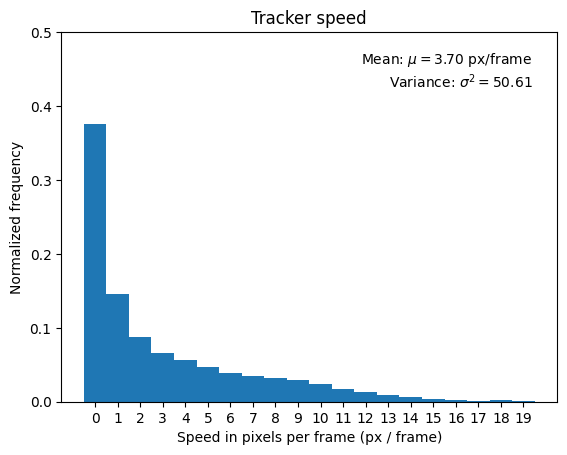
\includegraphics[width=\textwidth]{figures/06_results/da/TrackerSpeed.png}
		\caption{\footnotesize{Probabilistic representation of the speed of the ants within a sequence processed by the best tracker.}}
		\label{fig:tracks_speed_tck}
	\end{subfigure}
	\begin{subfigure}[]{0.45\textwidth}
		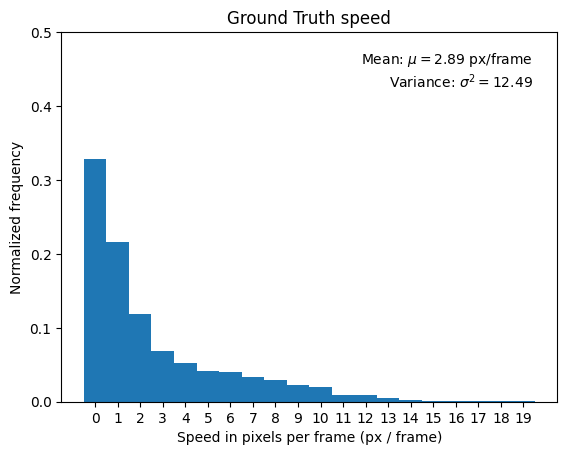
\includegraphics[width=\textwidth]{figures/06_results/da/GroundTruthSpeed.png}
		\caption{\footnotesize{Probabilistic representation of the speed of the ants within a ground truth sequence.}}
		\label{fig:tracks_speed_gt}
	\end{subfigure}
	\caption[Ants speed Normalized histogram]{\footnotesize{Comparison of the probabilistic representation of the speed of the ants between the best tracker and the ground truth.}}
	\label{fig:tracks_speed}
\end{figure}

\begin{figure}[!hp]
    \centering
    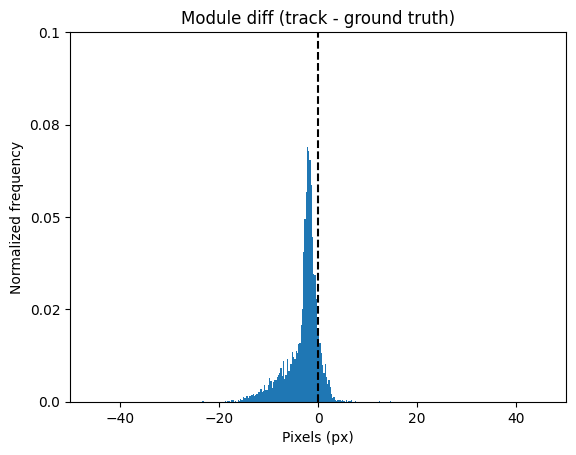
\includegraphics[width=0.45\textwidth]{figures/06_results/da/ModuleDiffTrack.png}
    \caption[Asymmetric error in tracker displacement]{\footnotesize{Asymmetric error in tracker displacement.}}
    \label{fig:tracker_module_diff}
\end{figure}

\needspace{0.1\textheight}

{
	Similar to the velocity, the location metrics computed with two consecutive bounding boxes within a track can be used in the study of the tracking results. 
	The histograms of \ac{IoU} can be seen in Figure \ref{fig:tracks_iou}, 
	comparing the ground truth with the tracker, it can be observed the tracker adapts correctly. 
	The histograms of \ac{CIoU} can be seen in Figure \ref{fig:tracks_ciou}, in these plots, 
	the distribution shifts towards higher scores compared to IoU. 
	The distribution shifts provides a smoother representation of the ground truth, making it easier for the tracker to reproduce the ground truth distribution, by instance, near the score value 1, where the ants are static.
}

\begin{figure}[!hp]
	\centering
	\begin{subfigure}[]{0.9\textwidth}
		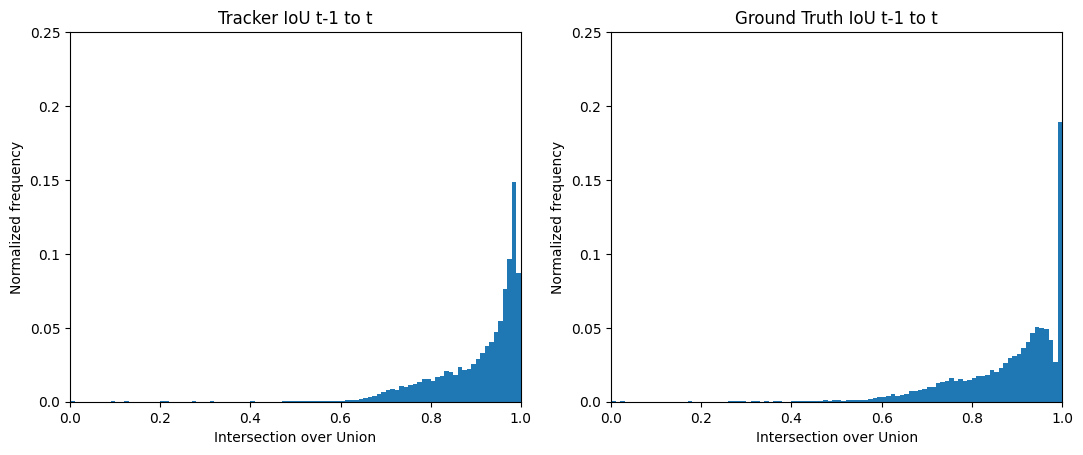
\includegraphics[width=\textwidth]{figures/06_results/da/Tracker_iou_vs_gt.png}
		\caption{\footnotesize{Comparison of the probabilistic representation of the IoU of the ants between the best tracker and the ground truth.}}
		\label{fig:tracks_iou}
	\end{subfigure}
	\begin{subfigure}[]{0.9\textwidth}
		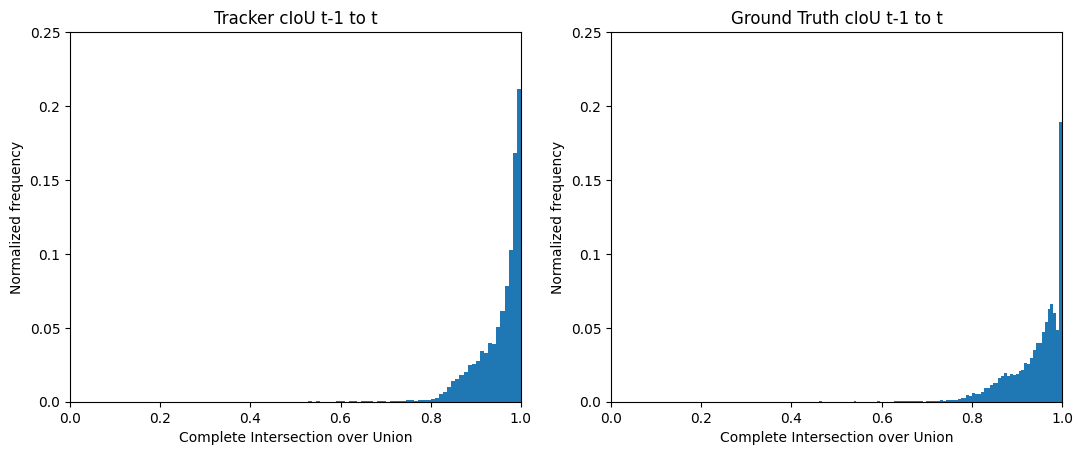
\includegraphics[width=\textwidth]{figures/06_results/da/Tracker_ciou_vs_gt.png}
		\caption{\footnotesize{Comparison of the probabilistic representation of the cIoU of the ants between the best tracker and the ground truth.}}
		\label{fig:tracks_ciou}
	\end{subfigure}
	\caption[Location metrics between frames]{\footnotesize{Comparison of the probabilistic representation of the the locations similarity within a track on the ground truth and the best tracker.}}
	\label{fig:tracks_location}
\end{figure}

\needspace{0.1\textheight}

{
	Figure \ref{fig:tracker_errors} and \ref{fig:tracker_iou_with_gt} were done by associating tracks and ground truth as explained in the HOTA subsection from the methodology section.
}

{
    From Figure \ref{fig:tracker_errors}, the right plot shows that the angular error of the estimated displacement is small, 
	a good explanation for the unsuccessful PCA model: adding complexity when it works will become a noisy source. 
	The left plot shows the module error of the estimated displacement is small, more detailed characterization was done at the beginning of this subsection (using module difference instead of module error).
}

{
	Figure \ref{fig:tracker_iou_with_gt} depicts the IoU of associated tracks and ground truth, 
	it is noticiable the valley at 0.8 IoU, which divides the data of a plot approximately in a 40\% at the left and a 60\% at the right. 
	Coinciding with the 60\% \ac{AssA} which measures the correct associations of observations and tracks.
}


\begin{figure}[!hp]
    \centering
    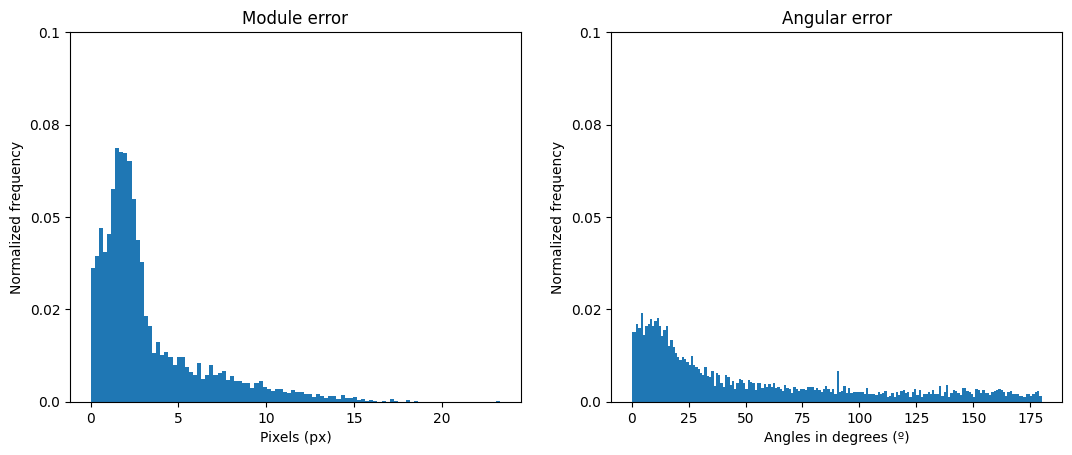
\includegraphics[width=0.9\textwidth]{figures/06_results/da/TrackerError.png}
    \caption[Displacement and angular error of the best tracker]{\footnotesize{The error in distance and angle of the best tracker.}}
    \label{fig:tracker_errors}
\end{figure}

\begin{figure}[!hp]
    \centering
    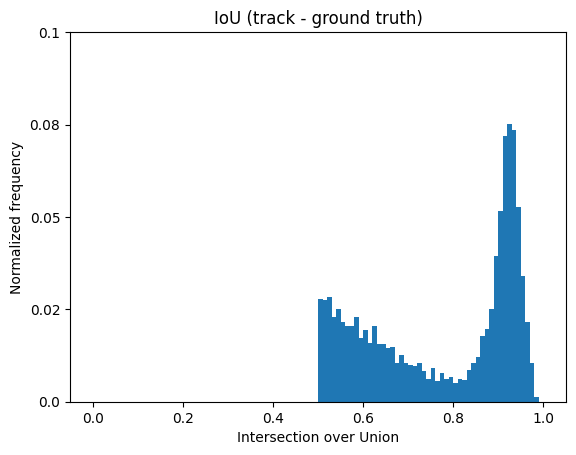
\includegraphics[width=0.45\textwidth]{figures/06_results/da/TrackerIoU_GT.png}
    \caption[Location similarity between the best tracking and the ground truth]{\footnotesize{Location similarity between the best tracking and the ground truth}}
    \label{fig:tracker_iou_with_gt}
\end{figure}

\FloatBarrier

%{
%    Finally, the HOTA metric is depicted in the Figure \ref{fig:tracker_hota_alpha}, 
%	and a 2D representation of a tracked sequence compared with its ground truth is shown in Figure \ref{fig:OCSORT_performance}, 
%	where each color line is a track and each row is a different identity.
%}
%
%\begin{figure}[!p]
%    \centering
%    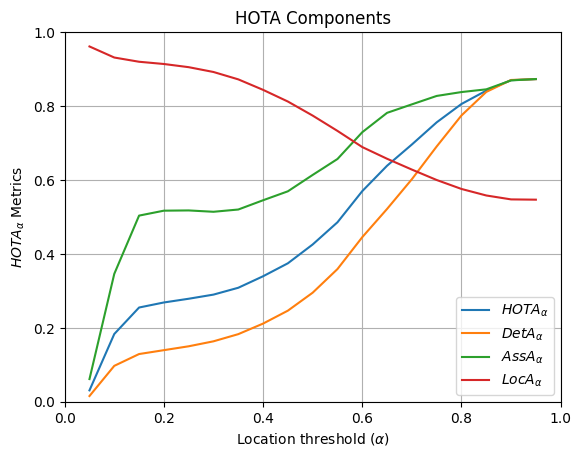
\includegraphics[width=0.9\textwidth]{figures/06_results/HOTA_componens.png}
%    \caption[Best tracker HOTA]{\footnotesize{HOTA partial components in function of the threshold for the best tracker.}}
%    \label{fig:tracker_hota_alpha}
%\end{figure}
%
%\begin{figure}[!p]
%	\centering
%	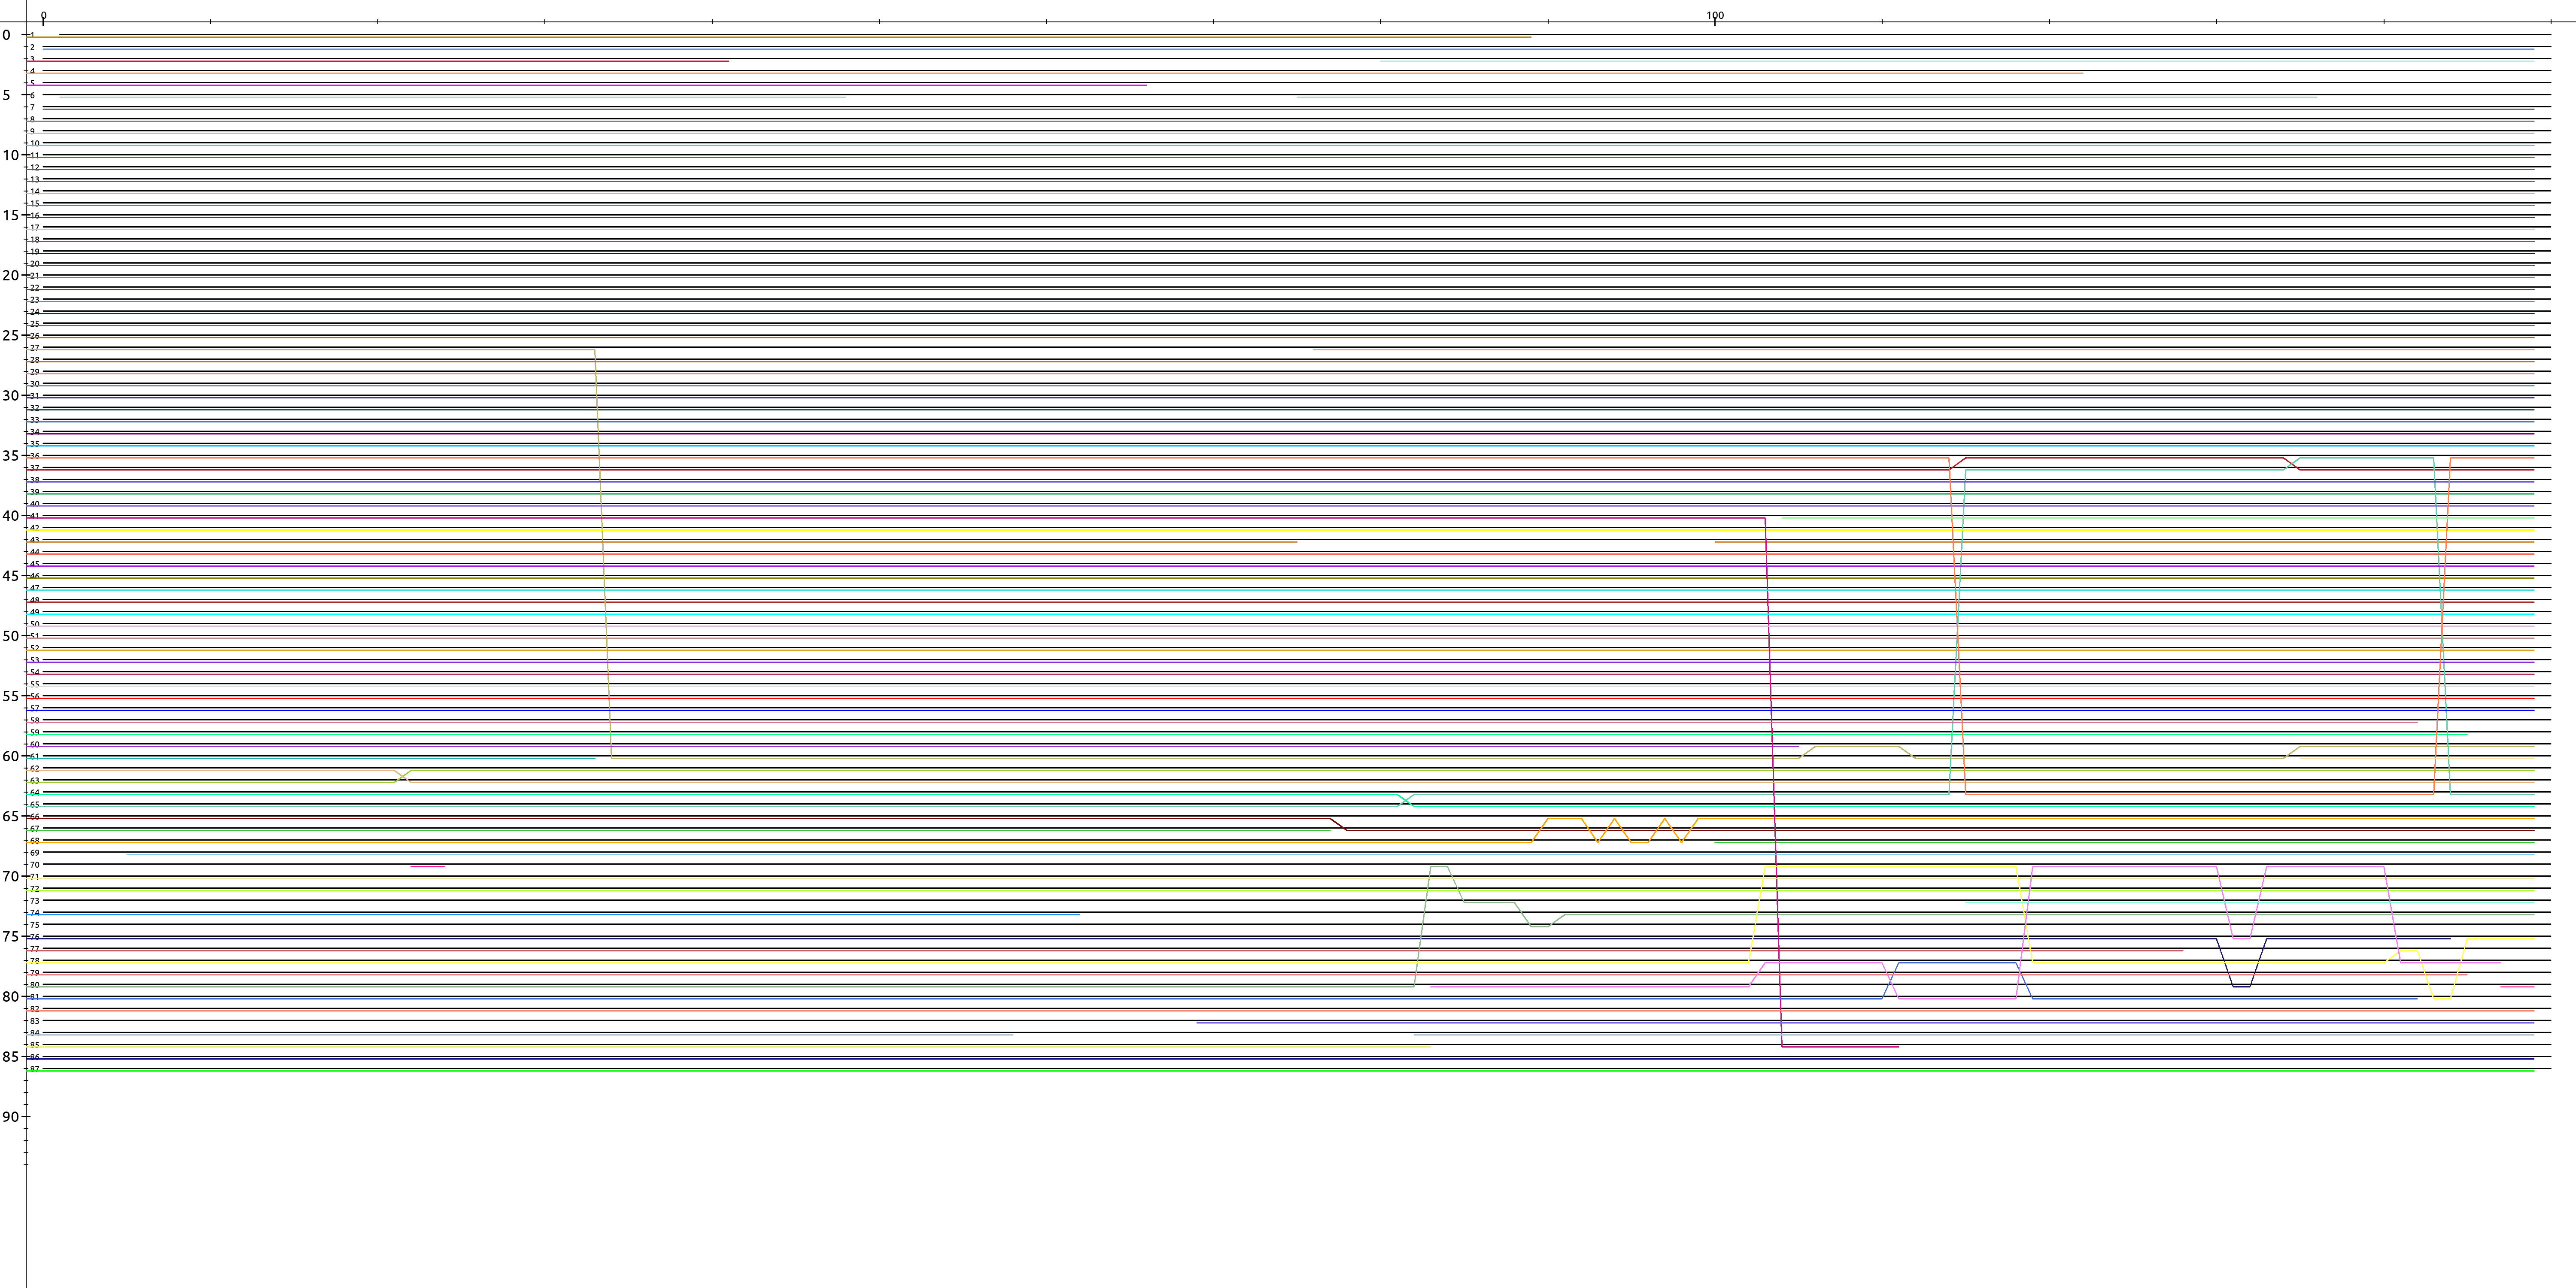
\includegraphics[width=0.9\textwidth]{figures/06_results/da/ocsort-results.png}
%	\caption[Visual representation of the OCSORT results]{\footnotesize{Visual representation of the OCSORT results.}}
%	\label{fig:OCSORT_performance}
%\end{figure}
